\documentclass{article}

\usepackage[a4paper]{geometry} % document dimensions
\usepackage{amsmath} % multiline equation numbering
\usepackage{amssymb} % e.g. triangleq, checkmark
\usepackage{textcomp,gensymb} % \degree symbol
%\usepackage{bm} % bold symbols numbering
\usepackage{authblk} % author/affiliation block
\usepackage[T1]{fontenc} % support accents via UTF
\usepackage[titletoc,title]{appendix}
\usepackage{booktabs} % e.g. \toprule

\usepackage{graphicx} % support for graphics
\usepackage[hidelinks, backref=page]{hyperref} % hyperlinks and autoref
\hypersetup{
    pdfauthor={Nick Ackerley},
    pdfsubject={Engineering Seismology},
    pdftitle={An Open Model of Probabilistic Seismic Hazard Assessment for the Indian Subcontinent},
    pdfkeywords={seismology, hazard, India, OpenQuake}}
\usepackage{natbib} % bibliography support
\usepackage{adjustbox} % support for too-wide figures
\usepackage{caption} % support for captions of floats
\usepackage{capt-of} % support for captionof
\usepackage{subcaption} % support for multiple figures with captions
\providecommand*\hyphen{-} % dashed page numbers in bib
\usepackage{listingsutf8} % for syntax-highlighted code
\usepackage[usenames,dvipsnames]{xcolor} % e.g. RoyalBlue
\usepackage{fontspec} % support for setmonofont
\setmonofont{Ubuntu Mono}[Scale=MatchUppercase]

\usepackage{pdflscape} % rotate contents and page using "landscape"
\usepackage{afterpage} % allows text to flow around landscape page
\usepackage{multirow} % cells spanning rows in \crefs
\usepackage{array} % text wrapping in centered cells
\newcommand{\multicell}[3][c]{%
  \begin{tabular}[#1]{@{}#2@{}}#3\end{tabular}}
  
\usepackage{enumitem} % control list formatting
\setlist{noitemsep}

% allow figures to take up more of a page
\renewcommand{\floatpagefraction}{0.7}

% just call everything a "section", except an "appendix"
\renewcommand*{\sectionautorefname}{Section}
\renewcommand*{\subsectionautorefname}{Section}
\renewcommand*{\subsubsectionautorefname}{Section}
\newcommand*{\Appendixautorefname}{Appendix}

% set up back-references
\renewcommand*{\backref}[1]{}
\renewcommand*{\backrefalt}[4]{%
    \ifcase #1 (Not cited.)%
    \or        (Cited on page~#2.)%
    \else      (Cited on pages~#2.)%
    \fi}

\lstdefinelanguage{Ini}
{
    basicstyle=\ttfamily\footnotesize,
    breaklines=true,
    keepspaces=true,
    columns=fullflexible,
    morecomment=[s][\color{RoyalBlue}\bfseries]{[}{]},
    morecomment=[l]{\#},
    morecomment=[l]{;},
    commentstyle=\color{gray}\ttfamily,
    morekeywords={},
    otherkeywords={=,:},
    keywordstyle={\color{green}\bfseries},
}

%%% PREAMBLE

\begin{document}

\title{An Open Model of Probabilistic Seismic Hazard Assessment for the Indian Subcontinent}
\date{\today}

\setcounter{Maxaffil}{0} % compact author block
\author[1,2]{N. Ackerley}
%\author[3]{G. Weatherill}
%\author[3]{M. Pagani}
\affil[1]{Istituto Universitario di Studi Superiori, Pavia, Italy}
\affil[2]{Université Joseph Fourier, Grenoble, France}
%\affil[3]{Global Earthquake Model (GEM), Pavia, Italy}

\maketitle

\begin{abstract}
Open models enable peer review and collaboration; open models can be built upon.
\end{abstract}

\tableofcontents
\listoffigures
\listoftables

\section{Introduction}
\label{sec:Introduction}

In this work a seismic hazard model for peninsular India \cite{nath2012probabilistic} is implemented within the OpenQuake \citep{pagani2014openquake,crowley2015openquake} platform.

This report is intended to be archived with the input and output files necessary to replicate the results at \url{https://hazardwiki.openquake.org/}.
References to file names in the electronic data are shown in \texttt{typewriter} font, as are keywords specific to OpenQuake, such as \texttt{bGRRelative}.

\subsection{Seismic hazard in the Indian subcontinent}
\label{subsec:PshaIndia}

The study of seismic hazard in India has been progressing steadily, from deterministic studies \citep{bis2002criteria} to probabilistic seismic hazard assessment (PSHA) and from site-specific towards larger regional studies.
\cite{ashish2016probabilistic} gives an up-to-date overview of the importance and history of this work.
Of particular note is the fact that the Bureau of Indian Standards has not updated their seismic hazard zonation since 2002 \citep{bis2002criteria}.
\cite{nath2012probabilistic} summarize concerns with this standard (currently in force), including underestimation of hazard, application of single zone factor to regions with very different hazard, and lack of treatment of uncertainty.

Some studies have focused on the extreme hazard of the Himalayas \citep{Bilham2001} in the the northeast, including the Shillong plateau, \citep{Das2006} and northwest \citep{Mahajan2009}.
Other studies have focused on regions of lesser but nonetheless high hazard such as Gujarat \citep{Yadav2008} or considered the whole of stable ``peninsular India" \citep{jaiswal2007, ashish2016probabilistic}.
Only \cite{bhatia1999probabilistic} considered the whole of India, but as \cite{ashish2016probabilistic} points out, since it was part of a global hazard mapping project (GSHAP) it only included ``only a few sources for Peninsular India focusing on the inter-plate region along the Himalayan belt".

\cite{nath2012probabilistic} is thus distinguished from previous work in providing a detailed probabilistic hazard assessment for the whole of India, including neighbouring states such as Bangladesh and Nepal.
It is the culmination of several previous works, some unpublished, involving the same group of authors.
These works include development of a uniform catalogue \citep{nath2010earthquake}, development of ground-motion prediction equations (GMPEs) specific to the Shillong region \citep{nath2012ground}, evaluation of a suite of GMPEs applicable to India \citep{nath2011peak} and development of smoothed-gridded and areal seismicity models \citep{thingbaijam2011seismogenic}.
Although there are inevitably some limitations, as we shall see later, this work represents the current state-of-the-art as far as PSHA in the Indian subcontinent.

(In the discussion of possible improvements to \cite{nath2012probabilistic} it will be noted that while earlier investigations \citep{bhatia1999probabilistic, Das2006, Yadav2008, jaiswal2007} relied on areal seismogenic source zonation, \cite{nath2012probabilistic} adds smoothed-gridded point sources while \cite{ashish2016probabilistic} adds fault-modelling.
Different types of seismogenic zones address different types of hazard and return periods, and can be effectively combined using logic trees to better encapsulate epistemic uncertainty.)

\subsection{Open science and OpenQuake}
\label{subsec:Open}

The seismological research community is a collegial one: researchers generally share data, models, software and results freely.
However it is becoming generally recognized that scientific computation is falling short of expectations in terms of reproducibility \citep{fomel2009reproducible, donoho2009reproducible}.
As computing power grows, so do models and their complexity; it seems that our ability to describe these models is not keeping pace.
In other disciplines, the components of a properly-documented experiment are well-known and widely practised.
Scientific computing is a relative newcomer, and presents new challenges, such as the constant evolution of programming languages.

Reproducibility is one of the fundamental tenets of science.
In the context of scientific computing reproducibility requires, at a minimum, a complete description of model, software versioning and results, open source code, and access to sufficient computing power \citep{hinsen2011data}.

\cite{nath2012probabilistic} provides the majority of the model description and results as an electronic supplement.
Unfortunately this description is incomplete, and worse, the software used to run the simulations is not freely available.
The consequence is that results cannot be verified, errors cannot be corrected and improvements cannot be made.

OpenQuake \citep{pagani2014openquake} is a fully-featured suite of software for the modelling of seismic hazard and risk. 
It is based on the OpenSHA framework \cite{field2003opensha} but developed in the Python programming language.
The source code is open, freely distributable and modifiable, and version-controlled at \url{https://github.com/gem/}.
Input and output files are encoded using and XML schema called the Natural Hazard Risk Markup Language (NRML) and which is both human- and machine-readable. 
NRML input files are standardized and can be combined between projects; NRML hazard output files can become the input to subsequent risk analyses.
OpenQuake is an ideal platform for development of PSHA models.
In fact, there is an ongoing effort to build a Global Earthquake Model based on OpenQuake.

\subsection{Overview}
\label{subsec:Overview}

In \autoref{sec:Implementation} the process followed to translate the model of \cite{nath2012probabilistic} for OpenQuake is detailed.

\autoref{subsec:GmpeTree} uses the GMPE logic tree as an introduction to the tectonic subregions and associated GMPEs. Potential improvements in terms of subregion and GMPE selection are reserved for \autoref{app:AlternativeGmpes}.

Issues relating to tectonic region assignments are addressed in \autoref{subsubsec:Areal}.
Difficulties encountered in interpreting and implementing the smoothed-gridded seismicity models are detailed in \autoref{subsubsec:Smoothed} while recommendations for an improved smoothed-gridded model are made in \autoref{app:Catalogue}. 
Improvements to source modeling are proposed in \autoref{app:SourceModelImprovements}.

In \autoref{subsec:GMPEs} issues encountered in implementing ground motion prediction equations (GMPEs) are discussed.

The modelling of source frequency-magnitude distribution (FMD) uncertainty described in \cite{nath2012probabilistic} turned out to be unimplementable in the strictest sense in OpenQuake and possibly on any platform, so compromises made are described in \autoref{subsec:SourceTree}.

\autoref{subsec:Verification} verifies the current results against those of  \cite{nath2012probabilistic}.
In particular hazard curves and maps and tables of ground motion with various probabilities of exceedence are presented and evaluated.
Inconsistencies between the figures and electronic supplement of \cite{nath2012probabilistic} are discussed.
\autoref{subsec:Sensitivity} investigates the importance of the use of region-specific ground motion prediction via their impact on hazard levels.

\autoref{subsec:Discussion} briefly explores the possibilities for future work while reserving more detailed discussion for the appendices.

Finally \autoref{app:Jobs} gives an overview of model files and related source code.

\section{Implementation}
\label{sec:Implementation}

\subsection{Ground motion prediction logic tree}
\label{subsec:GmpeTree}

The GMPE logic tree conveys some of the complexity of predicting earthquake hazard in peninsular India, and provides a starting point for discussion of both tectonic subregions and the GMPEs associated with them. 
The logic tree diagrammed in  \citet[Figure~3]{nath2012probabilistic} is redrawn for clarity in \autoref{fig:GmpeTreeNath}.
The tectonic region names and GMPEs listed differ slightly from \cite{nath2012probabilistic} but are exactly as found in the NRML model input files (e.g. source models mapped in \autoref{fig:ArealSourceModel} and  \autoref{fig:SmoothedSourceModel}) and the OpenQuake source code.

\newgeometry{bottom=4cm} 
\begin{figure}
\begin{adjustbox}{center}
\includegraphics{gmpe_logic_tree.pdf}
\end{adjustbox}
\caption[Original GMPE logic tree]{GMPE logic tree of \cite{nath2012probabilistic}, as encoded in \texttt{\detokenize{gmpe_logic_tree.xml}}.
Middle column selects tectonic region types mapped in \autoref{fig:ArealSourceModel}.
OpenQuake GMPE class names and assigned weights are given on the right side.
GMPE characteristics are are summarized in \autoref{table:GMPEs}}
\label{fig:GmpeTreeNath}
\end{figure}
\restoregeometry

\citet[Figure~3]{nath2012probabilistic} show \cite{sharma2009ground} being used for normal faulting in the active shallow crust, but normal faulting is the only kind of faulting \textit{not} supported by \cite{sharma2009ground}. 
This was assumed to be an error made in the drawing of the logic tree rather than the actual implementation.
Thus \autoref{fig:GmpeTreeNath} shows \cite{sharma2009ground} given weight only in zones where strike-slip or reverse faulting are predominant.

Although model input files may be ``human-readable'' no textual format of a directed graph will be easy for a human to read.
This sort of error highlights the need for ways of visually diagramming logic trees directly from the model input files. 
A script for converting NRML logic trees to \LaTeX\space was developed for this study.

Assignment of specific zones to tectonic subregions is treated further in \autoref{subsubsec:Areal}.
In particular methods are discussed for distinguishing between dominant fault mechanisms in the shallow crust and selecting GMPEs for intraslab subduction in deeper layers.

\cite{delavaud2009information} point out that macroseismic intensity observations are more abundant than instrumental recording, and go on to demonstrate that they can be used almost interchangeably for the purpose of quantitative assessment of GMPE efficacy.
This is particularly important in areas of low seismicity or sparse instrumentation macroseismic intensity, such as India.
\cite{nath2011peak} have made good use of this fact, but \cite{nath2012probabilistic} appear to utilize their efficacy assessments imperfectly. 
This and other issues which could be addressed in future work in this area are addressed in \autoref{app:AlternativeGmpes}.

\subsection{Seismogenic sources}
\label{subsec:Sources}

The electronic supplement of \cite{nath2012probabilistic} provides most but not all of the information required to generate a complete source model, even when supplemented by the earlier unpublished work of \cite{thingbaijam2011seismogenic} which focuses specifically on source modelling.
This section thus focuses on bridging the gaps to construct a complete source model.

\cite{nath2012probabilistic} proposed three source models: a single set of areal seismogenic source zones, and two smoothed-gridded point source models.
Combining these models using a logic tree (as discussed in \autoref{subsec:SourceTree} and diagrammed in  \autoref{fig:SourceTreeSymbolic}) allows the benefits of each model to be combined.
All models are derived from the catalogue of \cite{nath2010earthquake} for sub-catalogues with different minimum magnitudes and depth ranges.

Since some of these GMPEs are new to OpenQuake (see \autoref{table:GMPEs}) a comparison was done between the full model and that obtained with only the standard GMPEs.
For this purpose a "simplified" GMPE logic tree was constructed which simply omitted the newly-implemented GMPEs and used equal weighting for the rest. This is shown in \autoref{fig:GmpeTreeSimplified} and will be discussed in \autoref{subsec:Sensitivity}.

\subsubsection{Model layers}
\label{subsubsec:Layers}

\cite{thingbaijam2011seismogenic} divide their model into four layers as summarized in \autoref{table:Completeness} and \autoref{fig:DepthHistogram}.
Crustal thicknesses vary significantly across the region of study, but the convenience of constant model layer thicknesses turns out to be not entirely unrealistic.
The continental crust is 75-80~km thick beneath the Himalayas where the tectonics can be divided into shallow crust and interface \citep{thingbaijam2011seismogenic}.
Similarly in the the Shillong plateau of Northeast India the crust is quite thick and significant variation of stress drop with depth has been noted, with devastating ``pop-up'' type events \cite{bilham2001plateau} being generated in the lower crust \citep{nath2012ground}.
In stable continental regions the crustal thickness is a more usual 35-45~km, with seismicity concentrated in the uppermost 25~km.
The preceding seismotectonic features can be represented reasonably well using two seismogenic layers: 0-25~km and 25-70~km.

\begin{table}[!htb]
\centering
\caption[Summary of layer characteristics used for source models.]{Summary of layer characteristics used for source models.
Completeness magnitudes and years used in generating original smoothed-gridded seismicity models are from Table 1 of \cite{thingbaijam2011seismogenic}.
Layer identifiers used throughout this report are indicated.
Tops and bottoms of layers have been taken as seismogenic depth limits.
Hypocentral depths listed are at mid-layer.}
\label{table:Completeness}
\begin{tabular}{cccccccccc}
\multicolumn{4}{c}{minimum magnitude} & \multicolumn{2}{c}{4} & \multicolumn{2}{c}{4.5} & \multicolumn{2}{c}{5.5} \\
\midrule
layer & \multicolumn{3}{c}{
\begin{tabular}{ccc}
\multicolumn{3}{c}{depth (km)}\\min.
& max.
& hypo.\\
\end{tabular}
} & start & end & start & end & start & end \\
\midrule
1 & 0   & 25  & 12.5 & 1994 & 2008 & 1964 & 2008 & 1903 & 2008 \\
2 & 25  & 70  & 47.5 & 1990 & 2008 & 1964 & 2008 & 1902 & 2008 \\
3 & 70  & 180 & 125  & 1996 & 2008 & 1964 & 2008 & 1914 & 2008 \\
4 & 180 & 300 & 240  & 1970 & 2008 & 1984 & 2008 & 1912 & 2008 \\
\bottomrule
\end{tabular}
\end{table}

Intra-slab subduction occurs in three or four broad zones: the Hindu-Kush and Pamir ranges in the north-west, the eastern Himalayas and Indo-Myanmar subduction zones in the north-east and the Sumatra-Andaman subduction zone in the south east.
Deep-seated seismicity only occurs in the first and last region.
The tectonics of the Indo-Myanmar region are a combination of oblique subduction, accretion and collision \cite{wang2014active}.
These tectonic zones are represented by two deeper seismogenic layers: 70-150~km and 150-300~km.

This stack of depth-limited seismogenic zones can crudely represent the fact that subduction events are generally spread over a dipping plane (see \autoref{fig:DepthVsDistance}).
The four-layer structure furthermore captures the fact that there are 4 clear modes in the distribution of depths (see \autoref{fig:DepthHistogram}).

\subsubsection{Areal zones}
\label{subsubsec:Areal}

Areal source models are appropriate when source mechanisms and seismicity rates are relatively uniform across a given area.
They can provide a sound basis for regional assessment of b-value, maximum magnitude and other key parameters of a frequency-magnitude distribution, as shown in \cite{thingbaijam2011seismogenic}.

Selection of GMPEs (and thus the implementation of GMPE logic trees, see \autoref{subsec:GmpeTree}) depends on correct assignment of tectonic region types.
The main difficulty in implementing the areal source model of \cite{nath2012probabilistic} was that although the authors' intentions were generally clear, tectonic region assignments were not made explicit.

In layer~1, the shallow crust, assignments were made for this study using a combination of the representative focal mechanisms reported by \cite{nath2012probabilistic} and fault maps such as the HimaTibetMap database \citep{styron2010database}.
Zones obviously dominated by subduction faults were assigned ``subduction interface''; for the rest the representative rake was used to distinguish between fault mechanisms, as is customary in GMPE implementations.

$$
\text{mechanism} = 
\begin{cases}
\text{reverse} & 
\text{if threshold} < \text{rake} < 180 - \text{threshold} \\
\text{normal} & 
\text{if threshold} < -\text{rake} < 180 - \text{threshold} \\
\text{strike-slip} & 
\text{otherwise}
\end{cases}
$$

A threshold of 30\degree\space was chosen, consistent with the OpenQuake implementations of \cite{boore2008ground, campbell2008nga, sharma2009ground} but not \cite{zhao2006attenuation} which uses 45\degree.
Since the representative focal mechanism was computed as the average of the moment tensors reported in the GCMT database weighted by magnitude it is biased in favour of the larger earthquakes \citep{thingbaijam2011seismogenic}.

In layer~2, the deep crust, most zones are assumed to be dominated by interface subduction, except those in the stable continental part of peninsular India.

Intraslab subduction is expected to be dominant in layers 3 and 4.
\cite{nath2011peak} shows that the efficacy of GMPEs varies greatly between the Pamirs in the north-west and the Indo-burman subduction zone in the north-east. Unfortunately, \cite{nath2012probabilistic} gives no hints as to how to treat intraslab subduction for sources in Andaman-Sumatra and in the eastern Himalayas.
In the end it was decided to treat \cite[Figure~3]{nath2012probabilistic} as if ``Indo-Myanmar'' was intended to include the Andaman-Sumatra subduction as well.
Thus one group of GMPEs is used for ``subuction Himalayas'' while another is used for ``subduction'' (i.e. everywhere else).

The inferred tectonic region assignments assumed are summarized in \autoref{fig:ArealSourceModel}.

\begin{figure}[!htb]
\begin{adjustbox}{center}
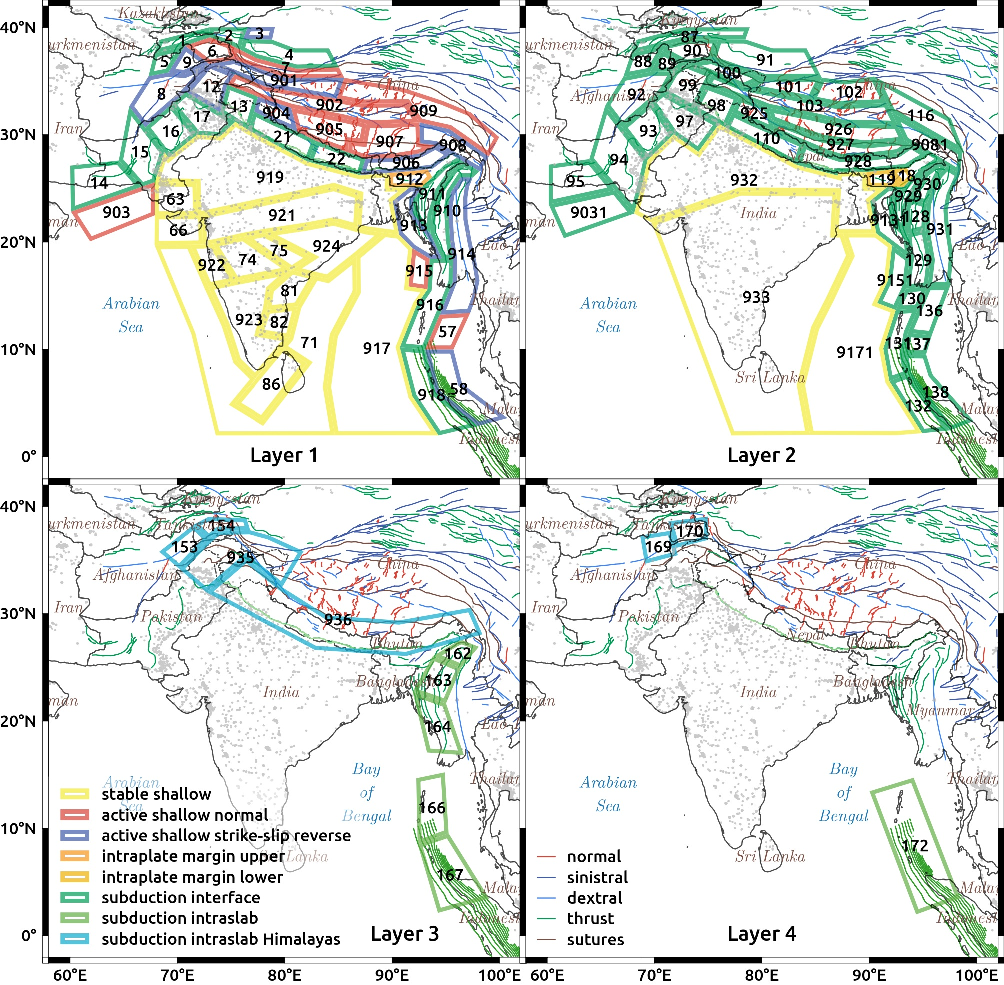
\includegraphics{India_Areal_Source_Model}
\end{adjustbox}
\caption[Areal source model]{Areal source model tectonic region assignments used in GMPE logic tree.
The areal source models is encoded in \texttt{\detokenize{areal_source_model.xml}}.
Zone identification numbers from \cite{nath2012probabilistic} are indicated.
Fault traces are from HimaTibetMap-1.0 \citep{styron2010database} except the Sumatran subduction fault which is from SLAB~1.0 \citep{hayes2012slab1}.
Fault data from the stable regions of India is lacking.
Urban areas, ``contiguous patches of built-up land greater than 1~km²'' \citep{schneider2009new}, are indicated in darker grey.}
\label{fig:ArealSourceModel}
\end{figure}

Potentially problematic tectonic region type assignments include:
\begin{itemize}
\item Zone 17 at the edge of the Pamir ranges is arguably ``stable shallow crust'' but was assigned ``subduction interface''.
\item Zone 906 in the Great Himalayas just north of the Shillong plateau was assigned ``active shallow crust strike-slip reverse'' even though the main trace of the Himalayan subduction fault runs through it, because the representative focal mechanism is strike-slip.
\item Zones 903 and 915-918 are predominantly oceanic crust but have been assigned ``active shallow crust'' or ``subduction interface'' according to the dominant focal mechanism and fault types.
For example zone 903 includes the Murray Ridge and so exhibits predominantly normal faulting as expected for a spreading ridge.
It is classified for the purpose of GMPE selection as ``active shallow crust normal'', but is likely in reality to produce ground motions distinct from an active continental crust.
\item Zones 71, 86 on layer~1 and zones 9031, 9081, 9131, 9151 and 9171 on layer~2 have have $a$ values of zero and so were assigned a ``no seismicity'' type and omitted from the areal source model.
\item Zones 169, 170 and 172 on layer~4 capture seismicity at 180-300~km depth, but only \cite{youngs1997strong} and \cite{kanno2006new} support depths below 180~km (see \autoref{table:GMPEs}).
\end{itemize}

Zones numbered as ``9xx'' in \cite{nath2012probabilistic} represent the amalgamation of several zones from \cite{thingbaijam2011seismogenic}.
In some cases this was done because of similarity of source mechanisms and statistics while in others it was necessary because the amount of seismicity in one of the zones was insufficient for FMD characterisation.
Furthermore, zones numbered ``9xx1'' in layer~2 have effectively had their seismicity transferred to the corresponding zones 9XX in layer~1.
For example zones 32 and 115 in \cite{thingbaijam2011seismogenic} become zones 908 and 9081 in \cite{nath2012probabilistic}, where zone 9081 has no seismicity.

Note that on layers 3 and 4 two distinct tectonic region types are defined for intraslab subduction \citep[p.
137]{nath2012probabilistic}.
Specifically, the ``Indo-Myanmar and Andaman-Sumatra subduction zones'' are assigned ``intraslab'' while the ``Himalayas and northwest India-Eurasia convergence'' are assigned ``intraslab Himalayas''.
Different GMPEs are applied in these regions, as described in \autoref{subsec:GmpeTree}, in particular the Japan and Cascadia adjustments of \cite{atkinson2003empirical} are applied, respectively.

Magnitude-scaling relations are used in PSHA to determine the actual rupture dimensions once a magnitude has been drawn from a frequency-magnitude distribution.
These were relatively straightforward to select once the tectonic region assignments were made, since ``\cite{wells1994new} for crustal events and those given by \cite{strasser2010scaling} for the subduction earthquakes'' \citep[p.~140]{nath2012probabilistic}.
It was inferred that for interface and intraslab regions \texttt{StrasserInterface} and \texttt{StrasserIntraslab} should be used, respectively.
The comment that ``the fault-rupture area estimated from the magnitude is constrained by a factor of 2'' \citep[p.~140]{nath2012probabilistic} was similarly interpreted as a width/depth aspect ratio of 2.

Since it is not explicitly stated in \cite{nath2012probabilistic} the seismogenic depth was assumed to be midway between the minimum and maximum for each layer.
Potential refinements to this setup are discussed in \autoref{app:SourceModelImprovements}.

The supplementary information required to generate the fully specified areal source model from the electronic supplement files \texttt{polygonlay\%d.txt} and \texttt{seismicitylay\%d.txt} files in the is contained in \texttt{auxiliary data.csv}.

\subsubsection{Smoothed-gridded points}
\label{subsubsec:Smoothed}

Smoothed-gridded seismicity models aim to replicate geographic variations of activity rates in a catalogue-driven way.
Typically a smoothing kernel is used which enforces a correlation distance and limits the resolution.

Some details of the smoothing are contained in the unpublished \cite{thingbaijam2011seismogenic}: a Gaussian kernel was used, following the methodology of \cite{frankel1995mapping} with correlation distances of 65 and 85~km for $m_{min}$ of 4.5 and 5.5 respectively.

After some discussion with K.
Thingbaijam it was decided that although the models are described as ``spatially varying annual activity rates'' \cite[p.~140]{nath2012probabilistic} the electronic supplement actually contains spatially smoothed total seismicity, i.e. number of events (per cell).
In order to convert this information to activity rates, i.e. number of events per year (per cell), it was necessary to obtain the duration of each sub-catalogue.
Fortunately this missing ingredient is summarized in \cite[Table 1]{thingbaijam2011seismogenic} and reproduced in \autoref{table:Completeness}.

Given the total seismicity $N$ and the length in years of the relevant catalogue $T$ (see \autoref{table:Completeness}) the annual rate $\nu$ for a given model is obtained using:
\begin{equation} \label{eq:SeismicityToActivity} 
\nu = N/T 
\end{equation}

In OpenQuake each point in the smoothed seismicity model is treated as a point source with a specified frequency-magnitude distribution: at a minimum $a$, $b$ and $m_{max}$ must be spedified.
\cite{nath2012probabilistic} indicate that ``$b$-value and $m_{max}$ remain fixed within the source zone''.
Thus in the present study for the smoothed seismicity model the parameters $b$ and $m_{max}$ of the truncated Gutenberg-Richter magnitude-frequency distributions are inferred from the areal source model zonation.
For points inside zones with non-zero $a$ values in the areal source model this is trivial; for points outside these zones the zone with the shortest perpendicular distance to the point was chosen.

\begin{figure}[!htb]
\begin{adjustbox}{center}
\includegraphics{India_Smoothed_Source_Model}
\end{adjustbox}
\caption[Smoothed seismicity point source model]{Tectonic region assignments and activity rates for smoothed seismicity point source model.
The smoothed seismicity source models are encoded in \texttt{\detokenize{smoothed_source_model_mmin4.5.xml}} and \texttt{\detokenize{smoothed_source_model_mmin5.5.xml}}}
\label{fig:SmoothedSourceModel}
\end{figure}

A gridded point source model also requires specification of  tectonic region type and source mechanism for the selection and implementation of GMPEs, as well as the uncertainty in the FMDs.
Thus the same procedure was used to assign tectonic subregion, rake, dip, strike, magnitude scaling relations, $\sigma_b$ and $\sigma_{m_{max}}$. For example the tectonic subregion assignments are shown for the smoothed-gridded model with $m_min$ = 4.5 in \autoref{fig:SmoothedSourceModel}.

The truncated Gutenberg-Richter magnitude-frequency distribution in OpenQuake implements

$$ \lambda(M \geq m) = 10^{a - b m} = e^{\alpha - \beta m} $$

Ignoring events below some threshold $m_{min}$, the annual rate becomes

$$ \lambda(M \geq m_{min}) = e^{\alpha - \beta m_{min}} e^{-\beta (m - m_{min})} = \nu e^{-\beta (m - m_{min})} $$

Thus to compute the $a$ value for a point source from the activity rate $\nu$ for a given magnitude threshold, we take into account the $b$ value for the zone as follows:

$$a = \log_{10}(\nu) + b m_{min} $$

Similarly to compute the activity rate for an areal source we can use

\begin{equation} \label{eq:ArealActivity} 
\nu = 10^a - 10^{b m_{min}}
\end{equation}

In order to verify that the smoothed and areal models are approximately equivalent to each other and the catalogue, annual activity rates were computed for each.
Areal activity rates were computed using \eqref{eq:ArealActivity}.
Smoothed model activity rates were computed by summing the seismicity for all points and then applying \eqref{eq:SeismicityToActivity}.
Catalogue activity rates were computed by querying the catalogue of \cite{nath2010earthquake} with appropriate minimum magnitudes and within the bounds of the areal source model.
Note also that events are only counted if the epicentre is within one of the zones of the areal model.
This was done on a layer-by-layer basis as well as over the whole model.

\begin{table}
\caption[Comparison of annual seismicity rates]{Comparison of annual seismicity rates for areal model, smoothed-gridded seismicity model and catalogue.
In each case the value shown is the average or expected number of events per year $\nu$ above the given minimum magnitude.
Catalogue events and smoothed-gridded point sources are only counted if the epicentre is within one of the zones of the areal model.}
\label{table:Rates}
\centering
\begin{tabular}{ccccccc}
\toprule
$m_{min}$ & \multicolumn{3}{c}{4.5} & \multicolumn{3}{c}{5.5} \\
source &  areal & smoothed & catalogue & areal & smoothed & catalogue \\
\midrule
layer   &      &        &         &       &          &           \\
1       &   80 &    130 &      54 &   8.4 &      4.1 &       3.1 \\
2       &   68 &    174 &      78 &  10.4 &      3.6 &       3.8 \\
3       &   36 &     89 &      40 &   2.9 &      1.7 &       1.6 \\
4       &   12 &     43 &      10 &   1.6 &      1.2 &       1.2 \\
total   &  194 &    435 &     182 &  23.3 &     10.6 &       9.7 \\
\bottomrule
\end{tabular}
\end{table}

The results are tabulated in \autoref{table:Rates}.
Both the areal and smoothed models tend to overestimate the seismicity in the catalogue.
Discrepancies between the areal model and the catalogue are likely an artefact of taking the total seismicity for a given zone, computing a frequency-magnitude distribution, and applying that FMD uniformly over the zone.
Discrepancies between the smoothed model and the catalogue cannot be explained by the smearing effect of the smoothing kernel, because this should result in smoothed seismicity rates lower than the catalogue rates when computed over the same area, whereas we observe smoothed seismicity rates which are higher.
Improvements to the smoothed seismicity model are proposed in \autoref{app:SourceModelImprovements}.

Other issues of note:
\begin{itemize}
\item Zones 9031, 9081, 9131, 9151 and 9171 on layer~2 have $m_{max}$ values values of zero.
These zones all the the smoothed seismicity points in or nearest to these zones on layer~2 were assigned the $m_{max}$ values from the corresponding zones on layer~1, namely zones 903, 908, 913, 915 and 917.
\item Given that the Japan/Cascadia regional adjustments are used for intraslab subduction, it is not clear why they are not also applicable for interface subduction.
\item Although the hazard maps in the electronic supplement are at 0.2° and the paper says the smoothed-gridded models are also at 0.2° they are in fact at 0.1°.
\autoref{fig:SmoothedSourceModel} shows the model at just 0.2° for convenience.
\end{itemize}

\subsection{Ground-motion prediction equations}
\label{subsec:GMPEs}

In order to evaluate seismic hazard across the Indian subcontinent it is necessary to consider a wide range of tectonic and crustal propagation regimes, including some which may be unique to the region. 
In all, \cite{nath2012probabilistic} uses 21 GMPEs from 17 references, summarized in \autoref{table:GMPEs}. 

\afterpage{\clearpage\newgeometry{margin=2cm} 
\begin{landscape}
\begin{table}
\caption[Ground motion prediction equations]{Ground motion prediction equations used in this study.
``N'' indicates that models were newly implemented in OpenQuake for the current study.
``S'' indicates that the model has since been superseded by an equivalent model from the same authors.
Among the databases used, ``ENA'' stands for eastern North America, and ``NGA'' stands for next generation attenuation.
The tectonic region ``Type'' uses the following abbreviations: ``active'' shallow crust, ``intraplate'' margin, ``stable'' continental crust, ``interface'' subduction and ``intraslab'' subduction.
$N_E$ and $N_R$ are the number of earthquakes and records in the database, respectively.
$H$, $M$ and $R$ are the ranges of depth, magnitude and distance over which the GMPE is considered by the authors to be valid. The component ``C'' for which the GMPE is defined can be ``H'' for unspecified horizontal, ``R'' for random horizontal, ``A'' for average of horizontals, ``M'' for median of horizontals ``G'' for geometric mean of horizontals rotated into most adverse (GMRotI50) \citep{boore2006orientation}, ``S'' for peak of square root of sum of squares of horizontals or ``V'' for vertical.}
\label{table:GMPEs}
\centering
\begin{adjustbox}{center=\pagewidth}
\begin{tabular}{llcc >{\centering\arraybackslash}m{20mm} >{\centering\arraybackslash}m{15mm} ccccccccc}
\toprule
OpenQuake class & Reference & N & S & Database & 
Type & $N_E$ & $N_R$ & \multicolumn{2}{c}{$H$ [km]} & \multicolumn{2}{c}{$M$} &  \multicolumn{2}{c}{$R$ [km]} & C \\
\midrule
\texttt{ToroEtAl2002} & \cite{toro2002modification} & & & 
ENA & stable & \multicolumn{2}{c}{simulation} &
   &    & 5.0 & 8.0 &    & 1000 & A \\
\texttt{Campbell2003} & \cite{campbell2003prediction} & & & 
ENA & stable & \multicolumn{2}{c}{hybrid} &
   &     & 5.0 & 8.2 &  0 & 1000 & A \\
\texttt{AtkinsonBoore2006} & \cite{atkinson2006earthquake} & & & 
ENA & stable & \multicolumn{2}{c}{simulation} &
 2 &  30 & 5.0 & 8.3 &    & 1000 & H \\
\texttt{RaghukanthIyengar2007} & \cite{raghukanth2007estimation} & \checkmark & & 
peninsular India & stable & \multicolumn{2}{c}{simulation} &
 5 &  15 & 4.0 & 8.0 &    &  300 & A \\
\texttt{BooreAtkinson2008} & \cite{boore2008ground} & & \checkmark & 
NGA-West1 & active & 58 & 1574 &
   &     & 5.0 & 8.0 &  0 &  200 & G \\
\texttt{CampbellBozorgnia2008} & \cite{campbell2008nga} & &  \checkmark & 
NGA-West1 & active & 72 & 942 &
   &     & 4.0 & 8.0 &  0 &  200 & G \\
\texttt{SharmaEtAl2009} & \cite{sharma2009ground} & \checkmark & & 
Himalayas \& Zagros & active & 16 & 201 &
   &     & 5.0 & 7.0 &    &  100 & A \\
\texttt{AkkarBommer2010} & \cite{akkar2010empirical} & & \checkmark & 
Europe \& Middle East & active & 131 & 532 &
   &     & 5.0 & 7.6 &  0 &  100 & A \\
\texttt{NathEtAl2012Upper} & \multirow{2}{*}{\cite{nath2012ground}} & \checkmark & & 
Shillong & intraplate & \multicolumn{2}{c}{\multirow{2}{*}{simulation}} &
 0 &  25 & 4.8 & 7.6 & \multirow{2}{*}{10} &  \multirow{2}{*}{100} & \multirow{2}{*}{V} \\
\texttt{NathEtAl2012Lower} & & \checkmark & & plateau & margin & & &
25 &  40 & 4.8 & 8.1 &    &      &   \\
\texttt{AtkinsonBoore2003SInter} & \cite{atkinson2003empirical} & & & 
global & interface & 80 & 1155 &
20 &  50 & 5.0 & 8.3 & 10 &  550 & R \\
\texttt{ZhaoEtAl2006SInter} & \cite{zhao2006attenuation} & & \checkmark & 
Japan & interface & 269 & 1520 &
25 &  50 & 5.0 & 8.3 &    &  300 & A \\
\texttt{AtkinsonMacias2009} & \cite{atkinson2009predicted} & & & 
Cascadia & interface & \multicolumn{2}{c}{simulation} &
   &     & 7.5 & 9.0 &    &  400 & R \\
\texttt{Kanno2006Shallow} & \cite{kanno2006new} &  \checkmark & & 
Japan & active \textit{or} interface &  83 & 3769 &
 0 &  30 & 5.5 & 8.2 &    &  450 & S \\
\texttt{Kanno2006Deep} & \cite{kanno2006new} & \checkmark & & 
Japan & intraslab & 111 & 8150 &
30 & 200 & 5.5 & 8.2 &    &  450 & S \\
\texttt{YoungsEtAl1997SSlab} & \cite{youngs1997strong} & & & 
global & intraslab & 164 & 480 &
50 & 229 & 5.0 & 7.8 & 10 &  500 & A \\
\multicell{l}{\texttt{AtkinsonBoore2003SSlabJapan}\\\texttt{AtkinsonBoore2003SSlabCascadia}} & \cite{atkinson2003empirical} & \checkmark & & 
global &  intraslab &                80 & 1155 &
50 & 100 & 5.0 & 8.3 & 30 &  550 & R \\
\texttt{ZhaoEtAl2006SSlab} & \cite{zhao2006attenuation} & & \checkmark &
Japan & intraslab & 269 & 1725 &
50 & 120 & 5.0 & 8.3 &    &  300 & A \\
\texttt{LinLee2008SSlab} & \cite{lin2008ground} & & & 
Northeast Taiwan & intraslab & 54 & 4823 &
39 & 161 & 4.1 & 6.7 & 40 &  600 & A \\
\texttt{Gupta2010SSlab} & \cite{gupta2010response} & \checkmark & & 
Indoburman Arc & intraslab & 3 & 56 &
91 & 148 & 6.3 & 7.2 &    &  375 & M \\
\bottomrule
\end{tabular}
\end{adjustbox}
\end{table}
\end{landscape}
\restoregeometry\clearpage}

Nine of these GMPEs were new to OpenQuake. 
These were implemented following the quality assurance procedures described in \cite{pagani2014openquake}. 
In this section the focus is on the necessity and appropriateness of these new GMPEs, as well as concerns which arose during their implementation.

In the process of the development of a GMPE specific to the Indian Himalayas, an area of rapid urbanization and elevated hazard \cite{sharma2009ground} excluded shallow India-Bangladesh and deep India-Burma border events from their database on the basis that PGA has different distance scaling.
This observation points to the necessity of different GMPEs for these types of events, in the former case a GMPE specific to the Shillong plateau \cite{nath2012ground} and in the latter case, one specific to Indoburman subduction \cite{gupta2010response}.

The Shillong plateau (zones 118 and 912 in \autoref{fig:ArealSourceModel}) is an example of a tectonic regime specific to India. 
Situated in between the Himalayan and Indoburman subduction zones it would be considered a stable crustal region were it not for the massive normal faulting events known to occur there.
The great Assam earthquake of 1897 destroyed buildings within several hundred~km.
The two main structures involved, the Dauki and Oldham faults, are capable of M > 8 plateau-building events with a recurrence interval of 3-8 kyr each \citep{bilham2001plateau}.
\cite{nath2012ground} notes stress drop apparently increasing with depth and models $\kappa$ using a database of recent and minor but well-recorded earthquakes, and uses this information to develop stochastic models for events in the upper and lower crust.
The simulations are of vertical rather than horizontal motion at a hard-rock site.

The GMPE of \cite{sharma2009ground} is intended for the Indian Himalayas but is based on data from both Zagros Mountains in Iran and the Himalayas.
The database included only a small number of events (see \autoref{table:GMPEs}), of which only a few were in the Himalayas, and none a result of normal faulting. 
Compared to the other models available for active regions it is the only one based on data from India.
It is furthermore a valuable addition to a logic tree in the Shillong plateau because unlike the other models available for that region, it is not based on stochastic simulation. The GMPE lacks a $M^2$ term and so \cite{cotton2006criteria} would counsel against its inclusion in a logic tree, but it is retained for lack of an alternative for the region. 
During implementation it was observed that it does not actually define coefficients for PGA so they were assumed to be the same as for the spectral acceleration at 0.04 s.

The GMPE of \cite{gupta2010response} is essentially a regionalization of \cite{atkinson2003empirical} for intraslab subduction. 
On the basis of a database of just three events, the constant term of \cite{atkinson2003empirical} was recalculated, leaving the distance, depth, magnitude and site amplification terms unchanged.

The GMPE of \cite{raghukanth2007estimation} was developed for the stable shallow crust of peninsular India using stochastic simulation.  
\cite{raghukanth2007estimation} actually describe three models based on regional variations in Q, for Koyna-Warna, southern India and western-central India, plus a model for all of peninsular India obtained by sampling the regional models in proportion to their landmass. 
It has been assumed that \cite{nath2012probabilistic} did not use the regional models. 
In implementing \cite{raghukanth2007estimation} typographical errors were identified in the coefficient Tables 2, 3 and 5 by comparing results obtained with the smoother published curves in Figures 3 and 5. 
The grossest error in Table 2(b) was fixed while 3 other errors causing a maximum error of approximately 10\% error were not fixed (see \url{ http://docs.openquake.org/oq-hazardlib/master/gsim/raghukanth_iyengar_2007.html}).

\cite{kanno2006new} specifies two models, for shallow and deep events, based on data predominantly from Japan. 
Rather than distinguishing between seismotectonic regimes, this GMPE gives appropriate scaling relations based on depth alone. 
Thus ``both crustal and subduction interface events fall into the category of shallow events'' (p. 883) where ``shallow'' is defined as a ``focal depth of 30~km or less'' (p. 883).
This flexibility allows the GMPE to be used for many tectonic regimes, although as discussed in \autoref{app:AlternativeGmpes} it should in future work be restricted to regions where it demonstrates good efficacy. 

\autoref{table:GMPEs} shows that layer~4 (180-300~km) is significantly deeper than deepest events used in regression for \citet[100~km]{atkinson2003empirical},\citet[161~km]{lin2008ground}, \citet[120~km]{zhao2006attenuation} and \citet[148~km]{gupta2010response}. 
Of the GMPEs used for interface subduction in layer~4 only \citet[229~km]{youngs1997strong} includes events in the correct depth range.
In future work it would be beneficial to identify GMPEs appropriate for use in the depth range of layer~4 (see \autoref{app:AlternativeGmpes}.

Oddly, \cite{kanno2006new} is specified to 200~km depth, but is only used for interface events (layer~2).
Given the poor efficacy of \cite{kanno2006new} in the Hidukush/Pamirs it makes sense that it should be omitted in the Himalayas, but not in the Indo-Myanmar subduction zone.

It should be noted, finally, that \cite{kanno2006new} is defined for the ``peak square root of the sum of squares of two orthogonal horizontal components in the time domain'' (p. 880). Since the peak value is taken after computing the vectorial sum of the horizontals this is different from the (similarly rare) ``vectorial addition'' of \cite{douglas2003earthquake} where the sum is taken after  peak values are located in the time domain. 
This ground motion intensity measure component is more conservative than choosing a random horizontal component or the average of the peak horizontal components, but it is less conservative than the aforementioned vectorial addition. 
\autoref{table:GMPEs} shows that GMPEs for many different ground motion components are mixed in \cite{nath2012probabilistic}; this practice is not unusual but if left uncorrected errors do propagate through to hazard curves, and the resulting aleatory uncertainty is under-estimated \cite{beyer2006relationships}. 
OpenQuake tracks the type of horizontal component measured in its base \texttt{GroundShakingIntensityModel} class, but  does not currently make the necessary corrections to the mean or standard deviation of the ground motion.

\subsection{Source model logic tree}
\label{subsec:SourceTree}

The source model logic tree is shown in symbolic form in \autoref{fig:SourceTreeSymbolic}.

\begin{figure}[!htb]
\begin{adjustbox}{center}
\includegraphics{source_model_logic_tree_symbolic.pdf}
\end{adjustbox}
\caption[Symbolic source model logic tree]{Symbolic source model logic tree of \cite{nath2012probabilistic}.}
\label{fig:SourceTreeSymbolic}
\end{figure}

\cite{nath2012probabilistic} accounts for the epistemic uncertainty in seismicity model parameters by estimating the standard deviations of $b$ and $m_{max}$ in each source zone and assigning weights to ±1 standard deviation for each source.
This results in a source model logic tree too large to represent on a page; just a portion of it is shown in \autoref{fig:SourceTreePartial}.

\begin{figure}
\begin{adjustbox}{center}
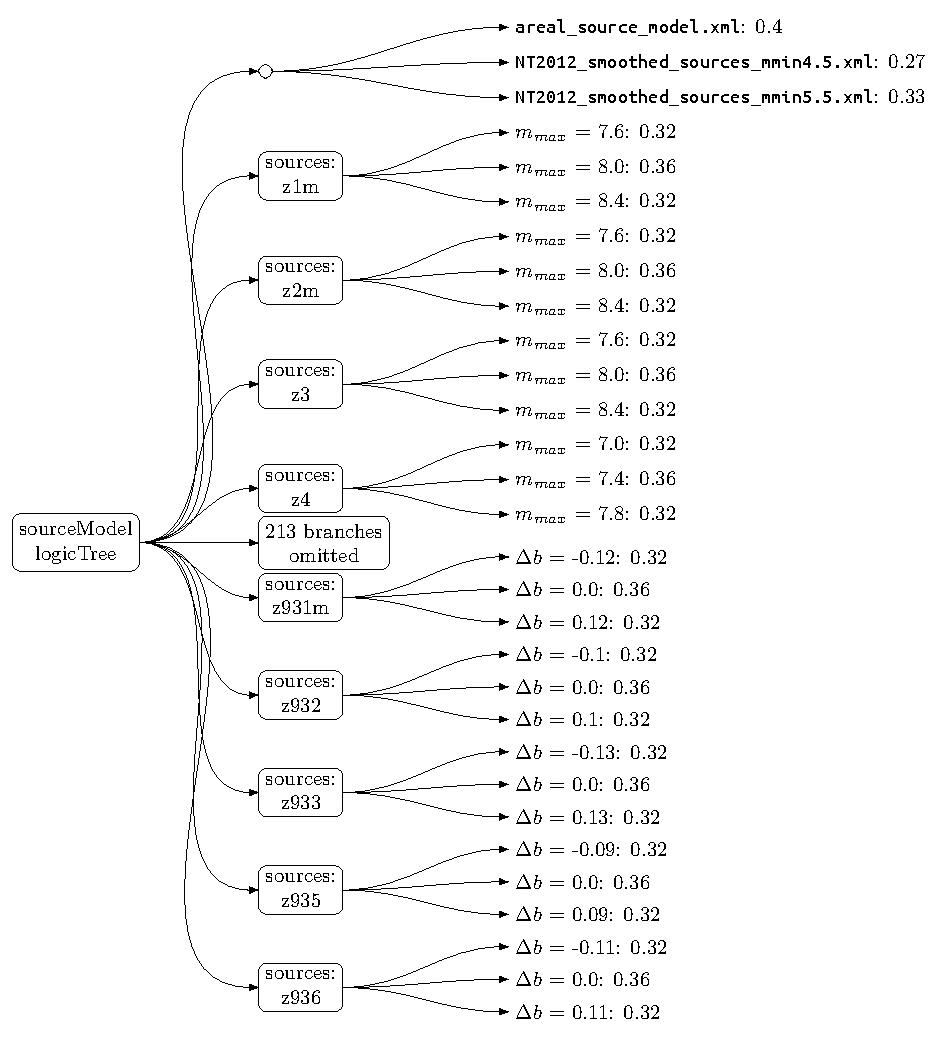
\includegraphics{source_model_logic_tree.pdf}
\end{adjustbox}
\caption[Partial source model logic tree]{Partial source model logic tree of \cite{nath2012probabilistic}.
The full model is encoded in \texttt{\detokenize{source_model_logic_tree.xml}}}
\label{fig:SourceTreePartial}
\end{figure}

Note that although Figure~4 of \cite{nath2012probabilistic} shows the activity rate $\nu$ (and by implication $a$) varying with $b$, no estimates of the standard deviation of $a$ or $nu$.
The  in OpenQuake happens to recalculate $a$ as $b$ After modifying $b$ using the uncertainty type \texttt{bGRRelative} the $a$ value is automatically recalculated to maintain constant total moment rate.
It has been assumed that this is the behaviour which \cite{nath2012probabilistic} implemented.

The fact that \autoref{fig:SourceTreePartial} has to be truncated is not simply a lack of page space.
Despite the common rendering of them in parallel, full enumeration actually takes place in series, so rather than just 3$\times$223 branches there are in fact $3^{223} \approx 10^106$, or just over a googol of branches.
Not only was full-enumeration out of the question, even partial enumeration was problematic on the current version of OpenQuake code.

It is unlikely that \cite{nath2012probabilistic} performed full-enumeration.
Some practitioners 

\section{Hazard results}
\label{sec:Results}

\subsection{Verification}
\label{subsec:Verification}

Validation of PSHA results would require comparison against observed hazard, and would require a much larger dataset than is currently available.
In this work we are merely verifying that the current model gives result close to those of \cite{nath2012probabilistic}.

\subsection{Sensitivity}
\label{subsec:Sensitivity}

\subsection{Discussion}
\label{subsec:Discussion}

\section{Conclusions}
\label{sec:Conclusions}

\section*{Acknowledgement}
Thanks to Kiran Thingbaijam for clarifications and engaging discussion.
Thanks to Amanda for your support.

\cleardoublepage
\phantomsection
\addcontentsline{toc}{section}{Bibliography}
\bibliographystyle{apalike}
\bibliography{/home/nick/Desktop/Library/PSHA.bib,/home/nick/Desktop/Library/india-hazard.bib}

\begin{appendices}

\section{Simplified GMPE logic tree}
\label{app:SimplifiedGmpeLogicTree}

A simplified logic tree used in initial studies is shown in \autoref{fig:GmpeTreeSimplified}.

\begin{figure}[!htb]
\begin{adjustbox}{center}
\includegraphics{gmpe_logic_tree_omit_new.pdf}
\end{adjustbox}
\caption[Simplified GMPE logic tree]{Simplified GMPE logic tree employing only established OpenQuake models, as encoded in \texttt{\detokenize{gmpe_logic_tree_omit_new.xml}}.
See \autoref{fig:GmpeTreeSimplified} for complete description.}
\label{fig:GmpeTreeSimplified}
\end{figure}

\section{Alternative GMPE logic tree}
\label{app:AlternativeGmpes}

In this section, possible improvements to the GMPE logic tree of \cite{nath2012probabilistic} in future work are discussed.

An obvious upgrade to the GMPE logic tree of \cite{nath2012probabilistic} would be to use updated models, whenever they exist, as per the recommendations of \cite{cotton2006criteria}. 
For example, the NGA-West1 models of 2008 were superseded in 2014 by NGA-West2, and so the newer models should be used \cite{bozorgnia2014nga}. 
Models which have been superseded and should be updated are indicated in \autoref{table:GMPEs}. 
This is trivial to implement since the newer models have already been implemented in OpenQuake.

A less straightforward but nonetheless important improvement would be to select GMPEs and possibly also to assign weights using measures of GMPE efficacy.
\cite{delavaud2009information} point out that macroseismic intensity observations are more abundant than instrumental recording and go on to demonstrate that the two can be used almost interchangeably for the purpose of quantitative assessment of GMPE efficacy.
This is particularly important in areas of low seismicity or sparse instrumentation, such as India.
\cite{nath2011peak} have made good use of this fact, but \cite{nath2012probabilistic} appear to utilize their efficacy assessments only imperfectly. 

For example in \citet[Figure~3]{nath2012probabilistic} there is a branch for megathrust earthquakes, because the GMPE of \cite{atkinson2009predicted} demands it, but no regional distinctions are made. 
Yet \autoref{table:LLH} shows clear differences in GMPE efficacy between interface subduction in the Himalayas and in the Andaman-Sumatra subduction zone.

\begin{table}[!htb]
\centering
\caption[Relative efficacy of GMPEs for interface subduction.]{Relative efficacy of GMPEs for interface subduction in the Indian subcontinent.
Negative average sample log likelihood (LLH) scores are from \cite[Table 5]{nath2011peak} while weights are computed using \cite{delavaud2012testing}.}
\label{table:LLH}
\begin{subtable}[b]{0.45\textwidth}
\caption{Himalayas}
\centering
\begin{tabular}{lccc}
\toprule
   Model &     LLH &  weight &   DSI \\
\midrule
   KAN06 &  2.4190 &    0.19 &  12.2 \\
  NATH09 &  2.4280 &    0.18 &  11.5 \\
  ATBO03 &  2.5733 &    0.17 &   0.8 \\
  ZHAO06 &  2.6512 &    0.16 &  -4.5 \\
  LILE08 &  2.6789 &    0.15 &  -6.3 \\
   YOU97 &  2.7117 &    0.15 &  -8.4 \\
\bottomrule
\end{tabular}
\end{subtable}
~
\begin{subtable}[b]{0.45\textwidth}
\caption{Andaman-Sumatra}
\centering
\begin{tabular}{lccc}
\toprule
   Model &     LLH &  weight &   DSI \\
\midrule
  ATMA09 &  2.5644 &    0.30 &   1.4 \\
  MEPA10 &  3.3970 &    0.17 & -43.0 \\
  ATBO03 &  3.4345 &    0.16 & -44.5 \\
  PETE04 &  3.5942 &    0.15 & -50.3 \\
  ZHAO06 &  3.7918 &    0.13 & -56.7 \\
   KAN06 &  4.2216 &    0.09 & -67.8 \\
\bottomrule
\end{tabular}
\end{subtable}
\end{table}

It appears as though GMPEs for all megathrust earthquakes were chosen by taking the top four ranking GMPEs (by LLH) for events in the Himalayas. 
Many authors \citep{scherbaum2009model, nath2011peak, delavaud2012toward, anbazhagan2015selection} seem unduly interested in "ranking", i.e. constructing an ordered list of GMPEs.
This is not a horse race.
\cite{scherbaum2009model} suggests a way to turn an LLH score into a logic-tree weight and \cite{delavaud2012testing} developed the concept of ``data support index''.
Using these measures \autoref{table:LLH} shows that in the Himalayas the data support the models more-or-less equally, and so it would make no sense to omit \cite{youngs1997strong} or \cite{lin2008ground} on this basis.

A better method than applying an arbitrary LLH cutoff for pruning logic tree branches would be to apply the principles of mutual exclusivity and collective exhaustiveness \cite{scherbaum2009model}. 
Models should be excluded if they are very similar in their predictions, particularly if the methodology for producing them is similar. 
As an example, note that among the models applied in the stable shallow crust, all but \cite{raghukanth2007estimation} were developed for eastern North America, and all but \cite{campbell2003prediction} are based on stochastic simulations. 
Since \cite{atkinson2006earthquake} and \cite{toro2002modification} have similar methodologies and \cite{nath2011peak} show that they have similar LLH scores they are not mutually exclusive and in future work it would make sense to omit one, likely the latter since it has a slightly higher LLH. 
By the same token, the addition of a fully-empirical model (if it exists) would bring the set of GMPEs closer to being collectively exhaustive, as would improved models specific to peninsular India or its subregions.

Whereas a distinction is made in \cite{nath2012probabilistic} between intraslab subduction in the Himalayas and Indo-Burman subduction zones, none is made for interface subduction. 
\autoref{table:LLH} suggests that model efficacy does differ greatly between the two regions. 
While many models are equally supported for the data in the Himalayas, several, notably \cite{kanno2006new}, are used by \cite{nath2012probabilistic} where they are not well-supported by the data. 
Therefore, in future work it would be appropriate to select subduction interface GMPEs differently in the Himalayas, the Indo-Burman subduction zone and Andaman-Sumatra.

Care must be taken when using efficacy measures to assess GMPEs in seismically stable regions. 
For example, it is dangerous to recommend a GMPE for a regions on the basis of a single event.
One study which does just this is \citep{anbazhagan2015selection}.
In an extreme case they propose different logic tree weights for Anjar and Bhuj  even though the epicentres and depths were very close together.
In contrast \cite{nath2011peak} compute LLH for 7 regions (using 38 events total) and state that, ``individual events do not have significant number of observations to support a viable ranking basis.''
\cite{anbazhagan2015selection} furthermore seem to misuse the concept of data support index (DSI) by simply setting weights to zero when the DSI is negative.
In contrast \cite{delavaud2012testing} insist that the difference between DSIs is more diagnostic than the sign of a given DSI.

In summary, in future work it is recommended to:
\begin{enumerate}
\item Replace models which have been superseded, in particular update NGA-West1 models to NGA-West2.
\item Split both intra-slab and interface subduction into Himalayan, Indo-Burman and Andaman-Sumatran tectonic subregions.
\item Use efficacy measures to select GMPEs more rigorously.
\item Incorporate models using different methodologies and/or databases, e.g. the BC Hydro subduction model of \cite{abrahamson2016bc}.
\item Incorporate models using more region-specific models.
\item Prune models which are quite similar to those already used, e.g. \cite{toro2002modification}.
\end{enumerate}

\section{Catalogue evaluation}
\label{app:Catalogue}

\section{Potential source modelling improvements}
\label{app:SourceModelImprovements}

\begin{figure}[htb]
\begin{adjustbox}{center}
\includegraphics{Depth_histogram_(mainshocks)}
\end{adjustbox}
\caption[Depth histogram for mainshocks]{Depth histogram for mainshocks over magnitude 5.5.
Mainshock identification is that of \cite{nath2010earthquake}.
Seismogenic layer boundaries and hypocentral depths used in the current implementation are indicated as dashed and dash-dotted lines respectively.}
\label{fig:DepthHistogram}
\end{figure}

\begin{figure}[!htb]
\begin{adjustbox}{center}
\includegraphics{Depth_vs_distance_(mainshocks)}
\end{adjustbox}
\caption[Depth vs.
distance for mainshocks in regions with deep events]{Depth vs.
distance for mainshocks in regions with deep events.
Subregions are indicated on each map; top left is the Hindu-Kush and Pamir ranges in the northwest of India viewed from the east, top right is the Andoman-Sumatran subduction zone viewed from the south while bottom left and right are beneath the Indoburman range and viewed from the east and south respectively.
Sub-catalogues were selected for events over magnitude 5.5 within a rectangular box of latitude and longitude as indicated on each individual plot.
 Horizontal and vertical axes are plotted at different scales.}
\label{fig:DepthVsDistance}
\end{figure}

\begin{itemize}
\item Base hypocentral depths on actual seismogenic depth distribution as shown in \autoref{fig:DepthHistogram}.
Placing the hypocentral depth at the modes of the overall catalogue would be a minor improvement.
Better still would be to capture the mode or to construct an approximate distribution for each areal zone.
\item Model the main Himalayan thrust as a simple fault.
In particular \cite{berryman2014himalayan} breaks the fault into three segments and provides necessary details such as dip and depth limits.
No variation of dip with depth is given, which is perhaps unrealistic, but at least the result is simpler to model.
Not all of the slip is being taken up on the frontal thrust; there are second and third folds which take up significant amount of slip, but the first is the most important from the standpoint of risk.
\item Model the Oldham and Dauki faults under the Shillong plateau as simple faults \citep{Bilham2001}.
\end{itemize}

\section{Summary of electronic data}
\label{app:Jobs}

This is an appendix because if you're reading this then you should already have the zip file with all of this data.

\texttt{auxiliary data.csv} 

\lstinputlisting[language=Ini,caption=\lstname]{phase1-job.ini}

\end{appendices}

\end{document}